\documentclass[mathserif]{beamer} 
\usepackage{eulervm} %красивый математический шрифт - по желанию
\usepackage{ulem} %зачёркивания
\usepackage{bm} %особо жирный математический
\usepackage{schemata} %для красивых блочных переходов, пользуюсь редко
\usepackage{mathtools} %улучшенная работа с типографией в math mode
\setbeamertemplate{navigation symbols}{} %отключает управляющие символы в правом нижнем углу
\usefonttheme{professionalfonts}
\usepackage{cmap} %чтобы были работающие гиперссылки
\usepackage{makeidx,fancybox,tikz}
\usetikzlibrary{automata, positioning, arrows,patterns}
\usetikzlibrary{arrows.meta}
\usepackage{tempora} %по желанию -- русские штрифты с засечками

\mode<presentation>
{
  \usetheme{CambridgeUS} 
  \usecolortheme{dove} 
}
\usepackage[T1,T2A]{fontenc}
\usepackage[utf8]{inputenc}
\usepackage[english,russian]{babel}
\usepackage{amsmath,mathrsfs} %ещё больше математических символов
\usepackage{amstext}
\usepackage{graphicx,relsize}
\graphicspath{ {./../images/} }

\usepackage{color}
\definecolor{gray}{rgb}{0.4,.4,0.4} %здесь можно определить собственные цвета
\definecolor{grey80}{rgb}{0.8,.8,0.8}
\definecolor{grey90}{rgb}{0.9,.9,0.9}
\definecolor{grey95}{rgb}{0.95,.95,0.95}
\newcommand\redstroke{\bgroup\markoverwith
{\textcolor{red}{\rule[0.5ex]{2pt}{1.5pt}}}\ULon} %зачёркивание жирной красной чертой

\newcommand\reduline{\bgroup\markoverwith
{\textcolor{red}{\rule[-0.5ex]{2pt}{1.5pt}}}\ULon}%подчёркивание жирной красной чертой

\newcommand\bluline{\bgroup\markoverwith
{\textcolor{blue}{\rule[-0.5ex]{2pt}{1.5pt}}}\ULon}

\newcommand\bolduline{\bgroup\markoverwith
{\textcolor{white}{\rule[-0.5ex]{2pt}{1.5pt}}}\ULon}

\title[] {Follow-автомат (IlieYu)}

\author[Chipollino]{Лучшая команда разработчиков по ТФЯ} % :))
\date[] 
{2022 г.}
\subject{Computer Science}

\newcommand{\Lang}{\mathscr{L}} %макрос для языка регулярки или автомата
\def\logor{\mathrel{\vee}} %отрендеренные логические операторы (с правильными интервалами)
\def\logimpl{\mathrel{\Rightarrow}}
\def\Linearize{\mathtt{Linearize}} %названия операций интерпретатора записываем моноширинным
\def\First{\mathrm{First}} %названия прочих операций записываем обычным шрифтом, но не тем, который в math mode по умолчанию
\def\Last{\mathrm{Last}}
\def\Follow{\mathrm{Follow}}
\def\IlieYu{\mathrm{IlieYu}}
\def\Glushkov{\mathtt{Glushkov}}
\def\Thompson{\mathtt{Thompson}}
\def\RemEps{\mathtt{RemEps}}
\def\DeAnnote{\mathtt{DeAnnote}}
\def\Annote{\mathtt{Annote}}
\def\Minimize{\mathtt{Minimize}}
\def\logand{\mathrel{\&}}
\def\lognot{\mathop{\neg}}
\def\iff{\mathrel{\Leftrightarrow}}
\def\quantall#1{\mathop{\forall #1}}
\def\quantex#1{\mathop{\exists #1}} 
\def\alter{\ensuremath{\mathrel{\vert}}}%отрендеренные регулярные операторы 
\def\star{\ensuremath{^{*}}}%отрендеренные регулярные операторы 
\def\regexpstr#1{\mathtt{#1}}%буквы внутри регулярок переписываются в моноширинный
\newcommand{\Nat}{\mathbb N}
\newcommand{\empt}{\varepsilon} %пустое слово
\newcommand{\bottom}{\bot} %противоречие
\newcommand{\rar}{\rightarrow} %стрелка вправо. Для экономии букв.
\newcommand{\RegExp}{\mathcal{RE}} %макрос для обозначения множества всех регулярок
%в преамбулу можно и нужно добавлять свои макросы

\begin{document}

\maketitle
% descriptive documentation :section
\section{Основные понятия}
\begin{frame}{Follow-эквивалентность}
  \begin{block}{\bf Определение}
    Пусть $R$ --- регулярное выражение. Положим $follow(a_{i}) = \{a_{j} | \exists w, u(wa_{i}a_{j}u \in\Lang(R))\}$.

    Follow-эквивалентность: состояния автомата Глушкова $a_{i}$ и $a_{j}$ follow-эквивалентны, если $follow(a_{i}) = follow(a_{j})$, и либо $a_{i}$, $a_{j}$ оба финальные, либо они оба не финальные.
  \end{block} % descriptive documentation
\end{frame}

\section{Follow-автомат (IlieYu)}
% descriptive documentation : frame
\begin{frame}{Конструкция автомата Илия-Ю (или follow-автомата)}
  \begin{block}{\bf Алгоритм построения $\IlieYu(r)$}
    \begin{itemize}
      \item Построить автомат Глушкова ($\Glushkov$);
      \item Объединить follow-эквивалентные состояния.
    \end{itemize}
  \end{block} % descriptive documentation
\end{frame}

\begin{frame}{Пример Follow-автомата (IlieYu)}\only<3> {\vspace{-5pt}}
  \vspace{-5pt}
  \only<1-3> {
    Исходное регулярное выражение:

    \[(\regexpstr{a}\alter \regexpstr{b})\star\regexpstr{b}\] % the initial regexp placeholder displaystyle
  }
  \only<1> {
    Автомат Глушкова:

    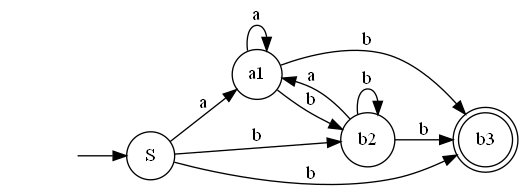
\includegraphics[width=4in, keepaspectratio]{follow1.png} % the Glushkov diagram placeholder
  }
  \only<2> {
    Follow-отношения:
    \begin{itemize}
      \item $S$: $a_{1}$ $b_{2}$ ; % the follow-relationships placeholder 1
      \item $b_{3}$: ; % the follow-relationships placeholder 2
    \end{itemize}
  }
  \only<3>{
    Follow-автомат:

    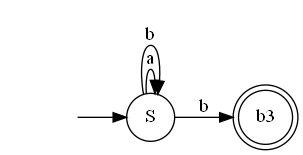
\includegraphics[width=3in, keepaspectratio]{follow2.png} % the IlieYu diagram placeholder
  }
\end{frame}

% overall documentation : section 
\section{Обсуждение}
\begin{frame}{Дополнительные сведения}
  \begin{block}{\bf }
    \begin{itemize}
      \item Меньше позиционного автомата и, в среднем, быстрее вычисляется.
      \item Может быть вычислен за квдратичное время.
      \item Является частным от позиционного автомата.
    \end{itemize}
  \end{block}
  \begin{block}{\bf Связь с автоматом Томпсона}
    Follow-автомат (IlieYu) может быть получен из автомата Томпсона путем последовательного применения к нему следующих операций:
    \[\DeAnnote(\Minimize(\RemEps(\Annote(\Thompson(r)))))\] % the formula IlieYu placeholder displaystyle
  \end{block}
  \begin{block}{\bf Теорема}
    Пусть $r$ -- взвешенное регулярное выражение над $K$. Если $K$ является $k$-замкнутым для автомата $\Thompson(r)$, то $\IlieYu(r)$ может быть вычислен за $O(mn)$ путем применения удаления $\empt$-переходов с последующей взвешенной минимизацией к  $\Thompson(r)$.
  \end{block}
\end{frame}
\end{document}
